\section{Analysis}\label{sec:analysis}
The analysis is divided into three different categories.
However, it should be said at this point that these categories will have overlaps.
Therefore, to avoid mentioning topics several times they will be mentioned only once.

\subsection{User}
The primary users for this application are persons with mental distress.
The question in this case is how is mental distress defined, or who is affected by it?
This question gets answered when looking into the core beliefs in the development of Woebot \cite{woebot-beliefs}.

\begin{quote}
    Everybody struggles sometimes. Cognitive distortions are something that everyone experiences in the context of strong emotion; it's part of being human.
\end{quote}

This quote shows clearly that not only persons with strong mental distress should consider using Woebot, but the application is for everyone.
The problem is that design for everyone holds the potential to exclude users by design\cite{feminist-technology}.
Designing for everyone is especially hard, because the human abilities and disabilities are a very wide range.
There are numerous counterexamples for users that do not fall into the extremely broad target group.
Everyone only includes persons being capable of the English language.
And even then it might be hard for persons with dyslexia to communicate with Woebot.\textcolor{red}{ Dyslexia cite}\\

\begin{figure}[ht]
    \begin{center}
        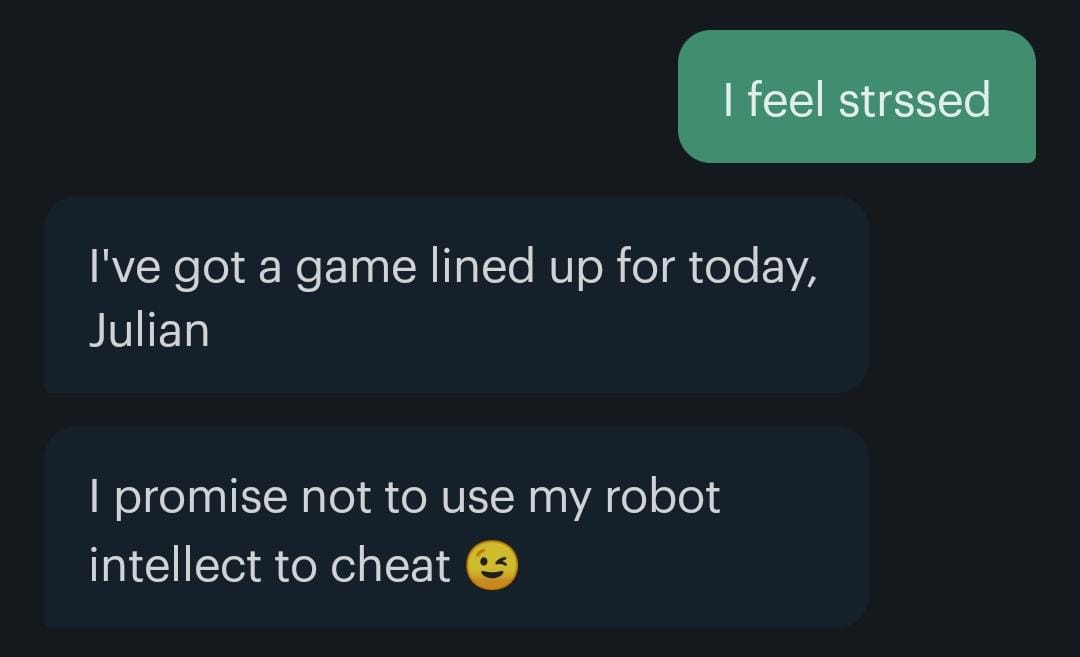
\includegraphics[width=1\columnwidth]{files/dyslexia.png}
        \caption{\label{fig:dyslexia} Cropped screenshot of a misunderstood call for help}
    \end{center}
\end{figure}

\autoref{fig:dyslexia} illustrates the problems that could happen when a typo occurs and Woebot can not understand the user correctly.
Woebot reacts inappropriate to a user trying to talk about being stressed.
Instead of helping Woebot misunderstands the user and continues suggesting a game, followed up by joking around.
This behavior obviously neglects the feelings of the user.
It has also been observed in a study conducted in 2020\cite{investigating-students}.
Not only did the users feel misunderstood, but the conversations felt repetitive.
Even more problematic is the fact that the user can not abort the current interaction and is forced to choose one of the predefined answers.\\

The figure also reveals the different problems with NLP, which will be further described in \autoref{sec:design}.
Typos could happen to many target groups.
People with cognitive or motoric disabilities could be affected by this.
A user group that may also not be considered are persons using a dialect of English and therefore be misunderstood.\\

A rather obvious counterexample is the general usage of the application.
It can only be accessed when the people wanting to use the application own a smartphone.
Although Woebot is capable of suggesting different lessons for relationships it is not capable for usage with more than one user.
The usage of the application is only limited to a single user.\\

% Human - AI Relations (Personification of Woebot?) - Concerns about therapeutic bond?

% How does it suggest to approach mental health? - Selfmanagement? Through Interaction?
% Norms and values: Culture sees mental problems as weakness -> Woebot doesn't solve this norm, it rather fights the weakness

% No gender?

% GIFs + Emojis - Personal but might be annoying/ not for every target group

\subsection{Design}\label{sec:design}
% Does it collect data, what does the app do with the data?

% Mood-Tracker:
% Not possible to click on emojis
% What looks like a prediction is actually none

% forced answers

% scrolling up - no jump down button

% Ai biased
% NLP - misunderstandings?
% NLP - users may not be aware of how much information a conversation shares
% Wrong calculations

\subsection{Context}
% Biometric sensor - privacy - phonesharing context
% Internet connection - Different contexts?
% Preload videos?

%%%%% General TODO %%%%%
% CEO & Founder explanation - Design with actors from the relevant field
